\documentclass{ieeeojies}
\usepackage{etoolbox}
\usepackage{cite}
\usepackage{amsmath,amssymb,amsfonts}
\usepackage{algorithmic}
\usepackage{graphicx}
\usepackage{textcomp}
\usepackage{array}
\usepackage[table]{xcolor}
\usepackage{multirow}
\usepackage{multicol}
\usepackage{float}

\def\BibTeX{{\rm B\kern-.05em{\sc i\kern-.025em b}\kern-.08em
    T\kern-.1667em\lower.7ex\hbox{E}\kern-.125emX}}





\begin{document}
\title{Using Forecasting Models in Cryptocurrency Price Prediction}

\author{\uppercase{Hoang Nhat Minh}\authorrefmark{1},
\uppercase{Le Nguyen Nhat Minh\authorrefmark{2}, and Tran Thi Luyen}\authorrefmark{3}}

\address[1]{Faculty of Information Systems, University of Information Technology, (e-mail: 21522336@gm.uit.edu.vn)}
\address[2]{Faculty of Information Systems, University of Information Technology, (e-mail: 21522338@gm.uit.edu.vn)}
\address[3]{Faculty of Information Systems, University of Information Technology, (e-mail: 21521107@gm.uit.edu.vn)}

\markboth
{Author \headeretal: Hoang Nhat Minh, Le Nguyen Nhat Minh, Tran Thi Luyen}
{Author \headeretal: Hoang Nhat Minh, Le Nguyen Nhat Minh, Tran Thi Luyen}

\begin{abstract}
Predicting cryptocurrency price has become a central focus for investors and traders in the rapidly evolving landscape of digital assets. Cryptocurrencies like Bitcoin, Ethereum, and other altcoins have captured global attention, with their prices subject to fluctuations influenced by various factors, from market sentiment to technological developments. With the unprecedented volatility of these markets, the need for accurate forecasting models has never been more crucial. In this research, we conduct an in-depth analysis using various models including Linear regression (LR), Autoregressive Integrated Moving Average (ARIMA), Recurrent Neural Network (RNN), Gated Recurrent Unit (GRU), Long Short-Term Memory (LSTM), Seasonal Autoregressive Integrated Moving Average with eXogenous factors (SARIMAX), Neural Basis Expansion Analysis Time Series (NBEATS), Random Forest (RF) to predict cryptocurrency price and determine the effectiveness of each model.
\end{abstract}

\begin{keywords}
Cryptocurrency, price prediction, Bitcoin, Ethereum, Linear regression, ARIMA, RNN, GRU, LSTM, SARIMAX, NBEATS, RF.
\end{keywords}

\titlepgskip=-15pt

\maketitle

\section{Introduction}
\label{sec:introduction}
Cryptocurrency, a digital form of currency, has transformed the traditional concept of money. Unlike cash, cryptocurrencies exist purely in electronic form, utilizing encryption techniques for secure transactions. Bitcoin, the pioneering cryptocurrency introduced in 2009 by Satoshi Nakamoto, paved the way for a myriad of digital currencies that followed. The decentralized nature of cryptocurrencies means they operate without a central authority, using blockchain technology to record and verify transactions across a network of computers. This decentralization provides a level of transparency and security previously unseen in financial systems. As interest and adoption continue to grow, cryptocurrencies are reshaping the landscape of finance, offering individuals around the globe new avenues for transactions, investments, and financial freedom. \newline
By using forecasting models and machine learning algorithms to analyze historical data of Bitcoin, Ethereum, and BNB, the research objective is to provide valuable insights for investors and traders to forecast the cryptocurrency price movement. To evaluate the performance of each predictive model, we use three metrics Mean Absolute Error (MAE), Mean Absolute Percentage Error (MAPE), and Root Mean Squared Error (RMSE).
\section{Related Works}
Mahir Iqbal and his team [1] applied a machine learning based time series analysis in predicting the price of Bitcoin. They used ARIMA, FBProphet, and XG Boosting for time series analysis and evaluated these models by using three parameters RMSE, MAE, and R Squared (R\textsuperscript{2}). After conducting the analysis, they concluded that ARIMA is the best of three with RMSE score and MAE score are 322.4 and 227.3 respectively.\newline
Harsha Nanda Gudavalli and Khetan Venkata Ratnam Kancherla [2] identified four machine learning algorithms RF, Gradient Boosting (GB), LSTM, and GRU to make long-term predictions of cryptocurrency prices. Overall, LSTM is the most accurate model based on RMSE score of 0.01083, MSE score of 0.00011, and R Squared score of 0.80618.\newline
Junyi Zhu [3] applied LR for Bitcoin price prediction with the accuracy rate for training RSS and testing RSS are 94.6\% and 96.99\% respectively.\newline
Namrata Hemraj Gawali [4] developed predictive models to predict the price of Bitcoin using LSTM, Seasonal Autoregressive Integrated Moving Average (SARIMA), SARIMAX, and RNN. In conclusion, LSTM outperformed all other models with R Squared score of 0.9519, MAE score of 2476.68, MSE score of 10958440.29 and RMSE score of 3310.35.\newline
Alikhan Bulatov [5] used N-BEATS trained on Bitcoin daily, hourly, and up-to-the-minute data in comparison with LSTM and ARIMA. In this analysis, it is concluded that N-BEATS is the best model for forecasting the Bitcoin price with the RMSE score in daily, hourly, and minute data are 308.859, 59.303, and 13.678 respectively.
\section{Materials}
\subsection{Dataset}
This research focuses on analyzing cryptocurrency trends through three data sets of three cryptocurrencies:
\begin{itemize}
	\item BTC/USD
	\item ETH/USD
	\item BNB/USD
\end{itemize}
Those data sets are extracted from the website investing.com with the selected period from March 1, 2019, to March 1, 2024. 
Each data set contains 1828 data rows and has 6 attributes:
\begin{itemize}
	\item Price: The last transacted price in a day.
	\item Open: The opening price in a day.
	\item High: The highest price in a day.
	\item Low: The lowest price in a day.
	\item Vol: The total amount traded in a day.
	\item Change \%: The percentage change in the closing price compared to the previous day’s closing price.
\end{itemize}
\subsection{Descriptive Statistics}
\begin{table}[H]
	\centering
	\caption{BTC, ETH, BNB’s Descriptive Statistics}
	\begin{tabular}{|>{\columncolor{red!20}}c|c|c|c|}
		\hline
		\rowcolor{red!20} & BTC & ETH & BNB \\ \hline
		Count & 1828 & 1828 & 1828 \\ \hline
		Mean & 25,983.05 & 1,488.75 & 212.44\\ \hline
		Std & 16,801.607 & 1,160.628 & 171.7707\\ \hline
		Min & 3,715 & 107.58 & 9.28\\ \hline
		25\% & 10,255.075 & 256.75 & 25.3325\\ \hline
		50\% & 23,637.8 & 1,573.75 & 242.4\\ \hline
		75\% & 38,686.75 & 2,152.043 & 318.675\\ \hline
		Max & 67,520 & 4,808.09 & 676.12\\ \hline
	\end{tabular}
\end{table}

\begin{figure}[H]
	\centering
	\begin{minipage}{0.23\textwidth}
		\centering
		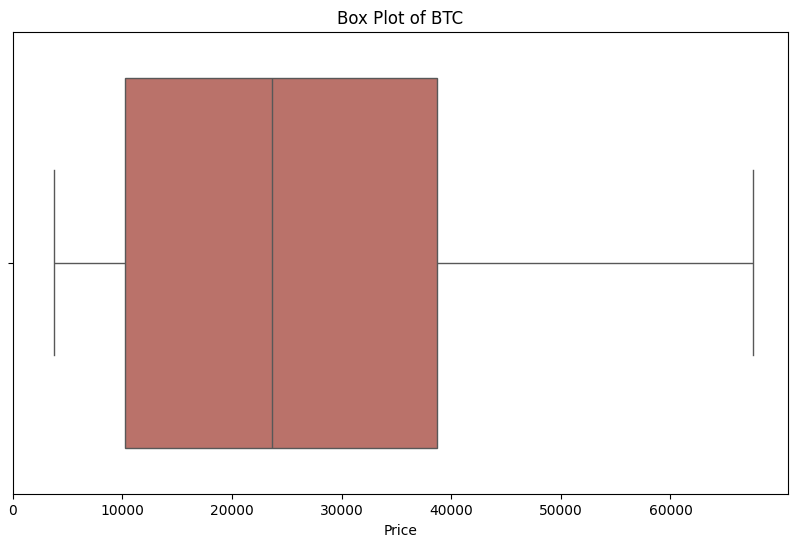
\includegraphics[width=1\textwidth]{bibliography/Figure/BTC_BoxPlot.PNG}
		\caption{Bitcoin price's boxplot}
		\label{fig:1}
	\end{minipage}
	\hfill
	\begin{minipage}{0.23\textwidth}
		\centering
		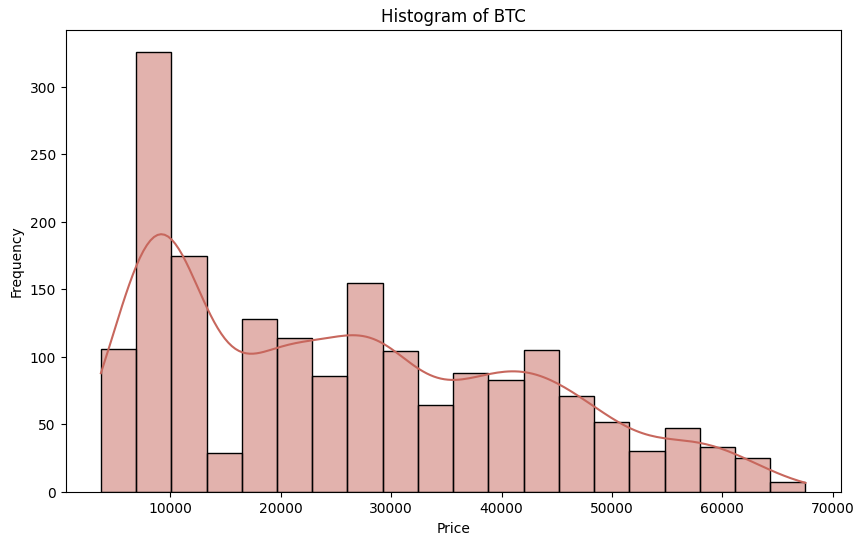
\includegraphics[width=1\textwidth]{bibliography/Figure/BTC_Histogram.PNG}
		\caption{Bitcoin price's histogram}
		\label{fig:2}
	\end{minipage}
\end{figure}

\begin{figure}[H]
	\centering
	\begin{minipage}{0.23\textwidth}
		\centering
		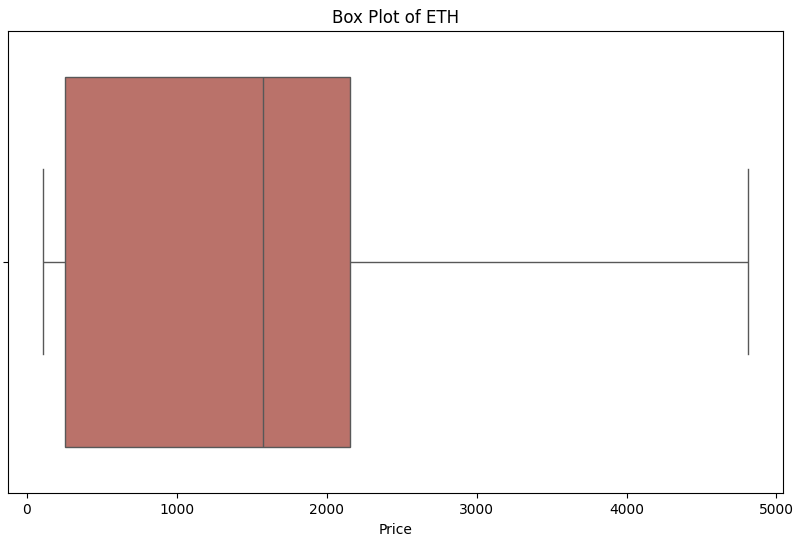
\includegraphics[width=1\textwidth]{bibliography/Figure/ETH_BoxPlot.PNG}
		\caption{Ethereum price's boxplot}
		\label{fig:1}
	\end{minipage}
	\hfill
	\begin{minipage}{0.23\textwidth}
		\centering
		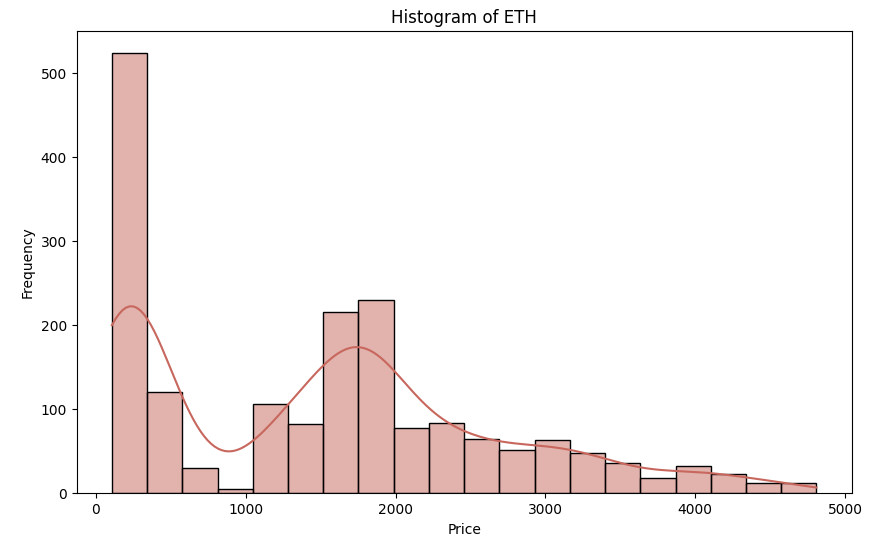
\includegraphics[width=1\textwidth]{bibliography/Figure/ETH_Histogram.PNG}
		\caption{Ethereum price's histogram}
		\label{fig:2}
	\end{minipage}
\end{figure}

\begin{figure}[H]
	\centering
	\begin{minipage}{0.23\textwidth}
		\centering
		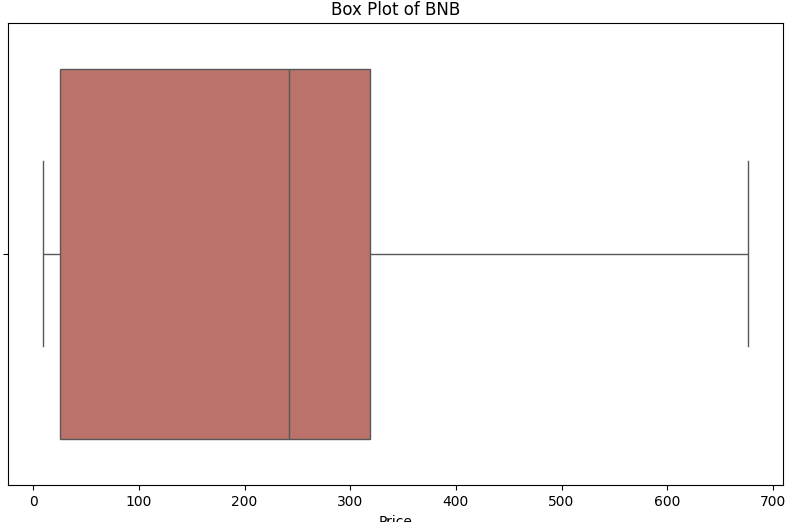
\includegraphics[width=1\textwidth]{bibliography/Figure/BNB_BoxPlot.PNG}
		\caption{BNB price's boxplot}
		\label{fig:1}
	\end{minipage}
	\hfill
	\begin{minipage}{0.23\textwidth}
		\centering
		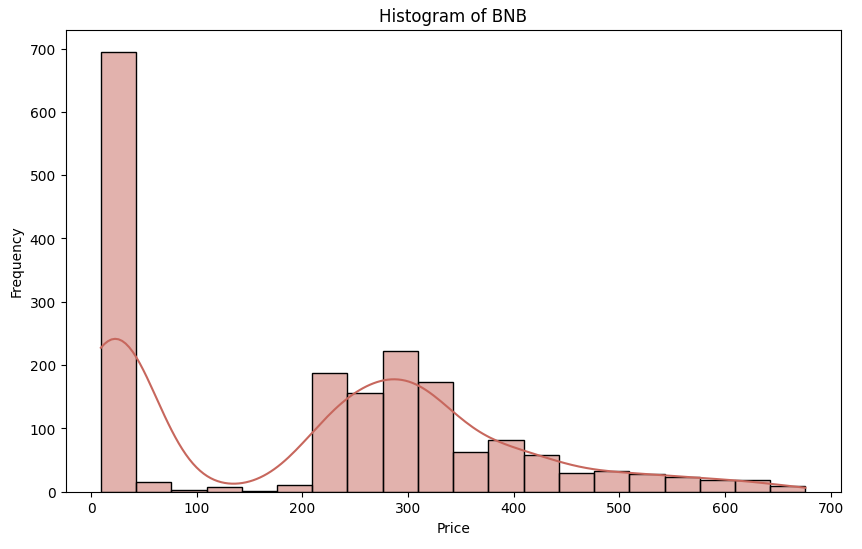
\includegraphics[width=1\textwidth]{bibliography/Figure/BNB_Histogram.PNG}
		\caption{BNB price's histogram}
		\label{fig:2}
	\end{minipage}
\end{figure}
\section{Methodology}
\subsection{Linear regression}
Linear regression is an algorithm that provides a linear relationship between an independent variable and a dependent variable. A linear regression model with more than one independent variable is called a multiple linear regression model. A multiple linear regression model has the form:
\newline  \centerline{$\textit{Y} = \beta_{0} + \beta_{1}X_{1} + \beta_{2}X_{2} + ... + \beta_{k}X_{k} + \varepsilon$}
\newline Where:
\begin{itemize}
	\item \textit{Y} is the dependent variable.
	\item $X_{1},...,X_{k}$ are the independent (explanatory) variables.
	\item $\beta_{0}$ is the intercept term.
	\item $\beta_{1},...,\beta_{k}$ are the regression coefficients for the independent variables.
	\item $\varepsilon$ is the error term.
\end{itemize}
\subsection{Autoregressive Integrated Moving Average (ARIMA)}
ARIMA is an acronym for AutoRegressive Integrated Moving Average. It is a statistical analysis model that uses time series data to either better understand the data set or to predict future trends. The full model can be written as:
\newline \centerline{$y'_{t} = c + \phi_{1}y'_{t-1} + ... + \phi_{p}y'_{t-p} + \theta_{1}\varepsilon_{t-1} + ... + \theta_{q}\varepsilon_{t-q} + \varepsilon_{t}$}
\newline Where:
\begin{itemize}
	\item $y'_{t}$ is the value of the time series at time t.
	\item \textit{c} is the constant term.
	\item $\phi_{1},...,\phi_{p}$ are the autoregressive coefficients.
	\item $\theta_{1},...,\theta_{q}$ are the moving average coefficients.
	\item $\varepsilon_{t}$ is the white noise at time \textit{t}.
\end{itemize}
A non - seasonal ARIMA model is classified as an ARIMA (p, d, q) model, where:
\begin{itemize}
	\item \textit{p} is the number of lag observations included in the model.
	\item \textit{d} is the number of times that the raw observations are differenced.
	\item \textit{q} is the size of the moving average window, also called the order of moving average.
\end{itemize}
\subsection{Autoregressive Integrated Moving Average with eXogenous factors (SARIMAX)}
SARIMAX is an acronym for Seasonal Autoregressive Integrated Moving Average with eXogenous factors. The SARIMAX model is an improved version of the SARIMA model, with exogenous factors  (X)  as  external  feature  parameters  for  enhancing  the  model’s  performance, reducing the prediction errors, overcoming the autocorrelation issues, and improving the prediction results. The SARIMAX model consists of both seasonal effects and exogenous factors that can be used as SARIMAX (p, d, q) * (P, D, Q), while the exogenous factors are optional parameters. The exogenous factors are used to support the prediction model and to provide it with more details. The SARIMAX model can be presented as:
\newline \centerline{$d_{t} = c + \displaystyle \sum_{n=1}^{p}\alpha_{n}d_{t-n} + \displaystyle \sum_{n=1}^{q}\theta_{n}\epsilon_{t-n} + \displaystyle \sum_{n=1}^{r}\beta_{n}x_{n_{t}}$}
\newline \centerline{$+ \displaystyle \sum_{n=1}^{P}\phi_{n}d_{t-sn} + \displaystyle \sum_{n=1}^{Q}\eta_{n}\epsilon_{t-sn} + \epsilon_{t}$}
\newline Where:
\begin{itemize}
	\item \textit{P} is seasonal autoregressive order.
	\item \textit{D} is seasonal differencing order.
	\item \textit{Q} is seasonal moving average order.
	\item \textit{s} is the length of the seasonal cycle.
\end{itemize}
\subsection{Random Forest}
Random forest is an ensemble learning method for classification, regression, and other tasks, that operates by constructing a multitude of decision trees at training time and outputting the class that is the mode of the classes (classification) or mean prediction (regression) of the individual trees.
\begin{figure}[H]
	\centering
	\begin{minipage}{0.23\textwidth}
		\centering
		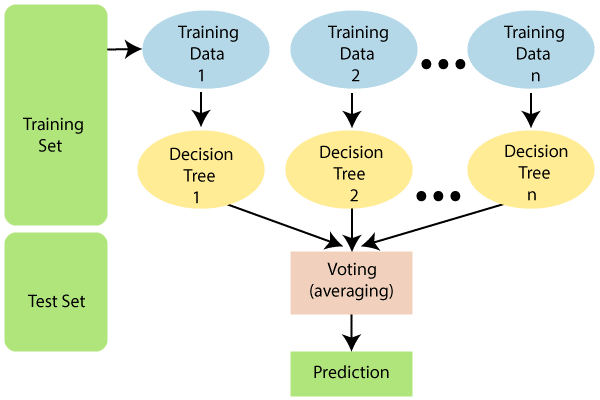
\includegraphics[width=1\textwidth]{bibliography/Images/RandomForest_Img1.png}
		\caption{The structure of Random Forest model}
		\label{fig:1}
	\end{minipage}
\end{figure}
Each tree in a random forest randomly samples subsets of the training data in a process known as bootstrap aggregating (bagging). The model is fit to these smaller data sets and the predictions are aggregated. Several instances of the same data can be used repeatedly through replacement sampling, and the result is that trees that are not only trained on different sets of data, but also different features used to make decisions.
\begin{figure}[H]
	\centering
	\begin{minipage}{0.23\textwidth}
		\centering
		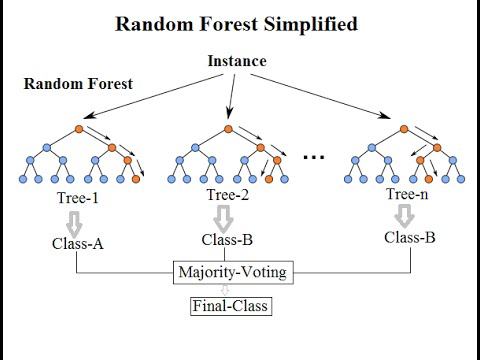
\includegraphics[width=1\textwidth]{bibliography/Images/RandomForest_Img2.png}
		\caption{Overview of Random Forest model}
		\label{fig:1}
	\end{minipage}
\end{figure}
The following steps explain the working Random Forest algorithm:
\begin{enumerate}
	\item Select random samples from a given data or training set.
	\item This algorithm will construct a decision tree for every training data.
	\item Voting will take place by averaging the decision tree.
	\item For classification, use majority voting; for regression, use averaging to derive the final output.
\end{enumerate}
\EOD

\end{document}
